\chapter{Results}\label{cp:results}

\begin{figure}[htpb]
    \centering
    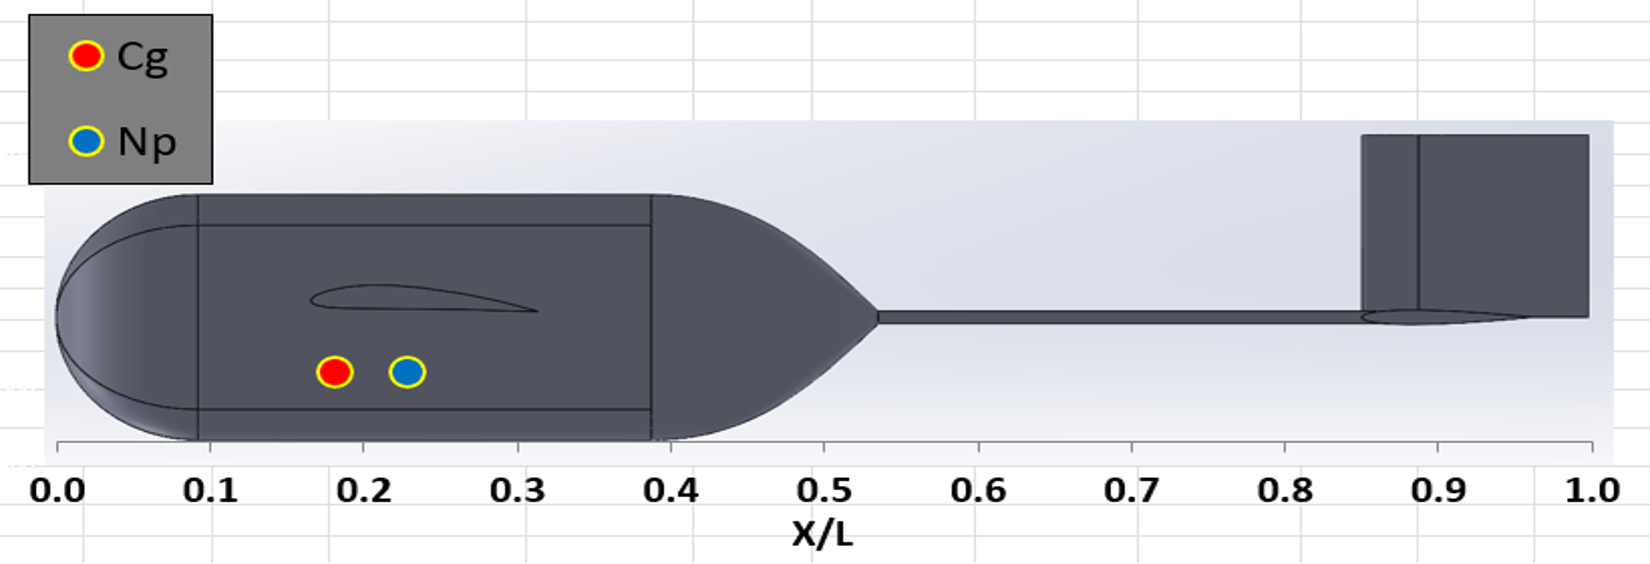
\includegraphics[width=\linewidth]{Figures/cg_np_side_view.png}
    \caption[\acrshort{cad} model with estimated \acrshort{cg} and \acrshort{np} locations]{Side profile visualization of the aircraft \acrfull{cad} model with estimated \acrfull{cg} and \acrfull{np} locations noted.}
    \label{fig:cg_np_side_view}
\end{figure}

\begin{figure}[htpb]
    \centering
    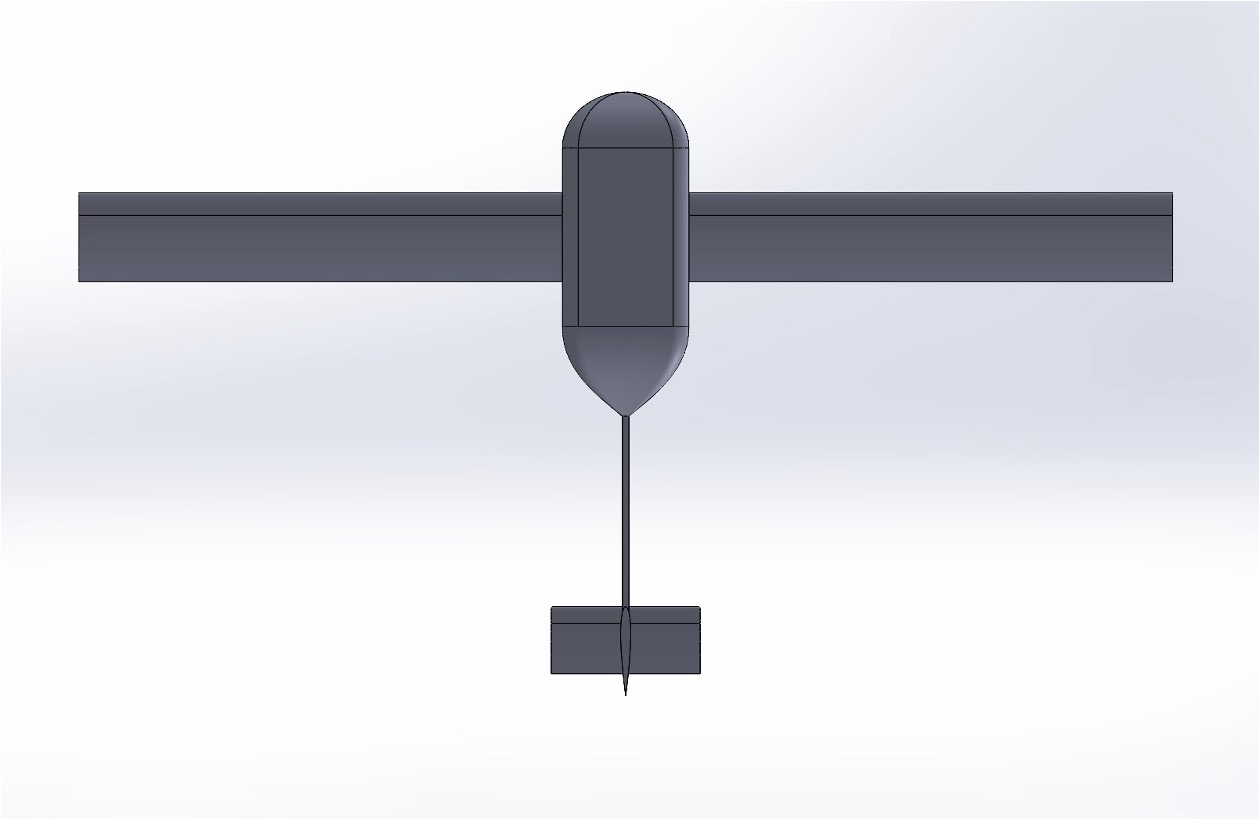
\includegraphics[width=0.9\linewidth]{Figures/top_view.jpeg}
    \caption[Top view of the \acrshort{cad} model]{Top view of the aircraft \acrshort{cad} model.}
    \label{fig:top_view}
\end{figure}

\begin{figure}[htpb]
    \centering
    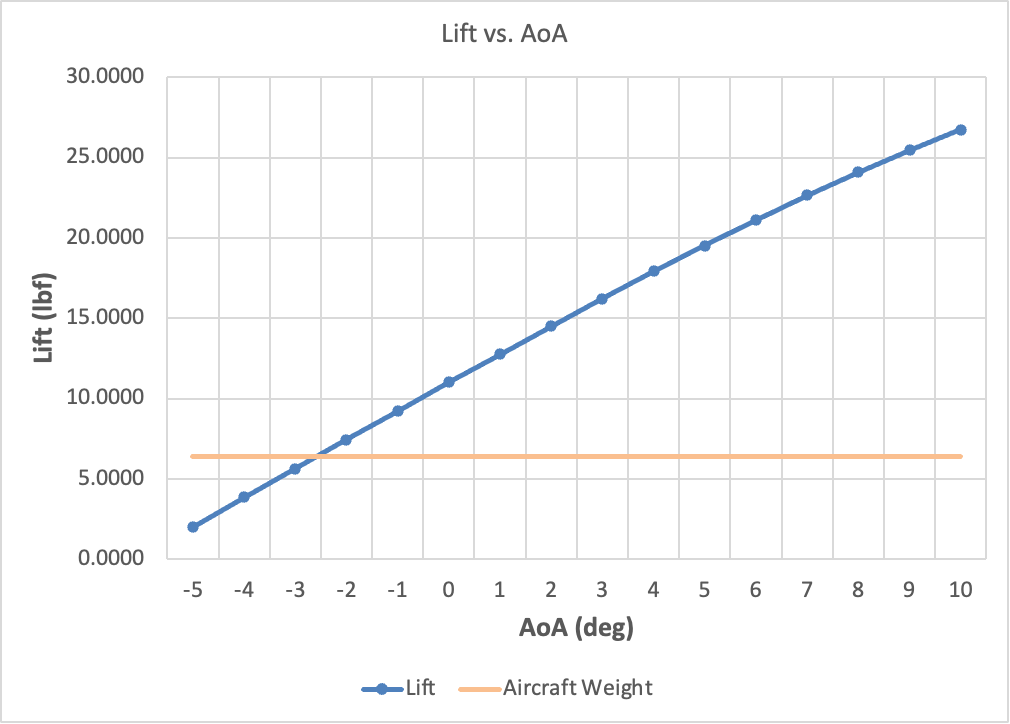
\includegraphics[width=\linewidth]{Figures/lift_vs_aoa.png}
    \caption[Lift vs. \acrshort{aoa}]{Lift force vs. \acrshort{aoa}, as reported by our STAR-CCM+ simulations.}
    \label{fig:lift_vs_aoa}
\end{figure}

\begin{figure}[htpb]
    \centering
    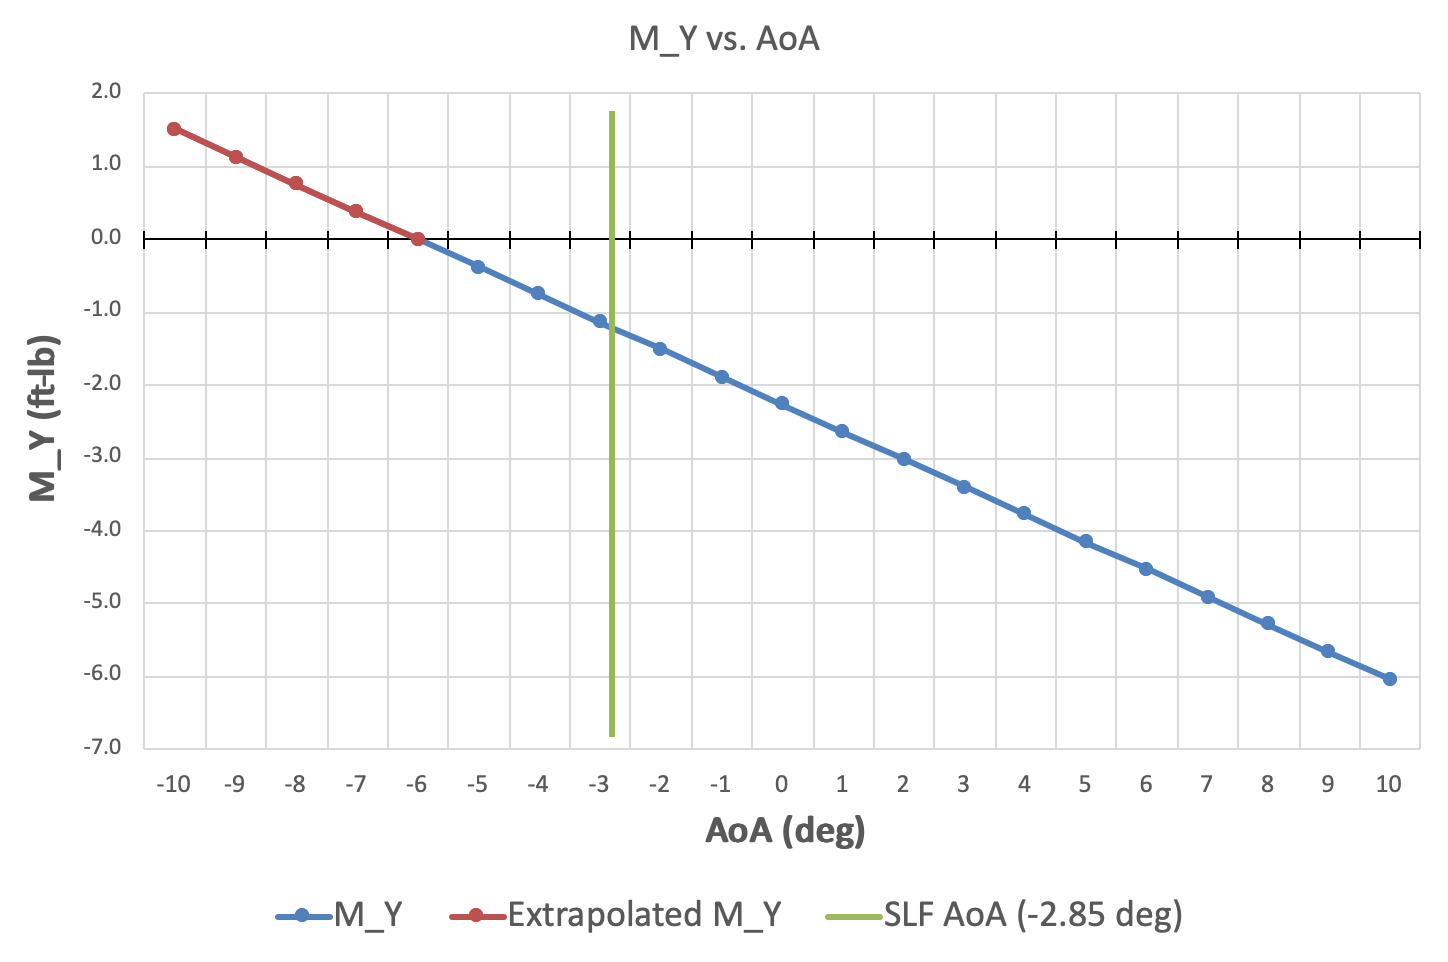
\includegraphics[width=\linewidth]{Figures/moment_vs_aoa.png}
    \caption[Pitching moment vs. \acrshort{aoa}]{Pitching moment vs. \acrshort{aoa}. Data at an \acrshort{aoa} less than \qty{-5}{\degree} is extrapolated since our analysis did not include this data, but we thought it would be pertinent to our report.}
    \label{fig:moment_vs_aoa}
\end{figure}
